\chapter{Introduction à la commande des systèmes robotisés}
\label{sec:introcommanderobots}

La science de "la commande" traite du développement d'algorithmes qui déterminent les actions qu'un système robotisé doit prendre en fonction de la situation pour atteindre un objectif (par exemple une position cible). Ces algorithmes sont généralement implémentés sur un micro-contrôleur, qui choisit les actions des actionneurs (par exemple le couple des moteurs électriques). Mathématiquement, le problème consiste à choisir les termes qui représentent les actions possible dans un système d'équations différentielles qui représentent le comportement du robot, afin d'obtenir le comportement désiré.

Lors de la conception des lois de commandes, plusieurs aspects peuvent être analysés selon le contexte: 

\paragraph{La stabilité} 

Lorsqu'une loi de commande est proposée, un critère essentiel dans la plupart des situations est la stabilité du système. La stabilité caractérise si les états du systèmes converge vers les états désirés ou bien si ils divergent. 

\paragraph{La faisabilité} 

Dans certain contextes, principalement ceux ou les actions possible sont limités (ex. couple maximum des moteurs), on s'intéresse tout simplement à savoir si il existe une séquence d'actions possibles qui peuvent permettre au système d'atteindre l'objectif. 

\paragraph{Le temps de réponse} 

La stabilité et la faisabilité détermine si le système pourra atteindre l'objectif. Ensuite, on cherche généralement à atteindre l'objectif le plus rapidement possible ce qui est caractérisé par le temps de réponse. Un critère relié est la "bande passante" du système, la "vitesse" du système exprimée dans le domaine fréquentiel.

\paragraph{L'optimalité} 

Il y a généralement un compromis à faire entre la vitesse (le temps de réponse) et l'utilisation agressive des actions possibles du système qui ont généralement un coût énergétique. Un objectif commun lors de la conception d'un asservissement est de maximiser la performance. La maximisation de la performance dans le domaine de la commande est généralement formulé comme la minimisation d'un coût qui combine les dépenses énergétiques et le temps passé loin de l'objectif.

\paragraph{La robustesse} Finalement, dans plusieurs situations il faut considérer l'incertitude dans le système lors de la conception des lois de commande. L'incertitude peut être due à des perturbations externes inconnues ou bien à des paramètres incertains du système robotique. L'analyse de robustesse consiste à vérifier si les lois de commandes vont fonctionner dans divers scénarios possibles. Des méthodes existe pour garantir le fonctionnement d'un contrôleur malgré un certain niveau d'incertitude (commande robuste ou commande adaptative).



\section{Illustration graphique à la conception de loi de commande}

À venir!

\section{Architectures}

Cette section introduits aux grandes catégories d'architecture de commande pour les systèmes robotisées. 


%%%%%%%%%%%%%%%%%%%%%%%%%%%%%%%%%%%%%%%%%%%%%%%%%%%%%%%%%%%%%%%%%%%%%%%%%%%%%%%%%%%%%%%%%%%%%%%%
\subsection{Boucle ouverte vs. boucle fermée}

La méthode de commande la plus simple est appelée boucle ouverte, voir Figure \ref{fig:openloop}. Par exemple, on détermine une séquence d'action pour les actionneurs (plan) qui va théoriquement faire bouger un système robotisé d'un point A au point B (objectif). Dans ce cas, la loi de commande est seulement une fonction du temps qui envoi les consignes pré-déterminés aux actionneurs. 
%%%%%%%%%%%%%%%%%%%%%%%%%%%%%%%%
\begin{figure}[htbp]
	\centering
		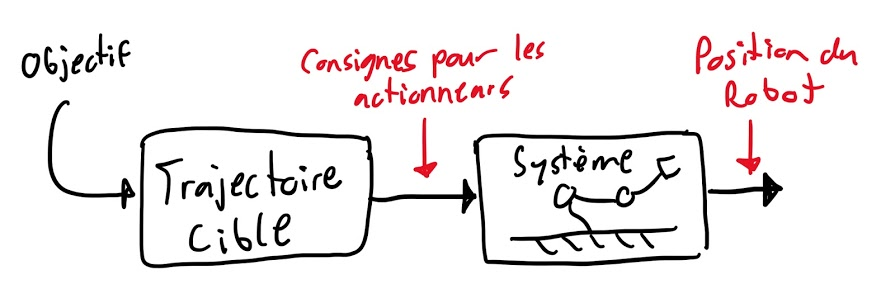
\includegraphics[width=0.7\textwidth]{fig/openloop.jpg}
	\caption{Boucle ouverte}
	\label{fig:openloop}
\end{figure}
%%%%%%%%%%%%%%%%%%%%%%%%%%%%%%%%

En général, cette méthode que l'on pourrait qualifier "d'aveugle" fonctionne seulement lorsque les systèmes ont très peu d'incertitude. Par exemple, une machine outil qui lit un code-G et traduit directement les instructions en consignes pour ses moteurs pas à pas est une approche purement boucle ouverte. Par contre, on peut facilement s'imaginer que cette approche ne fonctionnerait pas pour une voiture autonome qui doit aller d'une ville à une autre. Un voiture automne qui utiliserait un contrôleur basé sur une séquence d'angle de volant pré-déterminée divergerait rapidement de la trajectoire désirée du aux incertitudes. 

La plupart des contrôleurs utilisent une rétroaction continue basé sur des capteurs pour vérifier si le système évolue de façon approprié. C'est ce qu'on appelle l'approche boucle fermée,  illustré à la Figure \ref{fig:closedloop}. Dans ce cas, la loi de commande est une généralement fonction d'une erreur qui résulte de la comparaison de la position cible et la position réelle mesurée par des capteurs. 
%%%%%%%%%%%%%%%%%%%%%%%%%%%%%%%%
\begin{figure}[htbp]
	\centering
		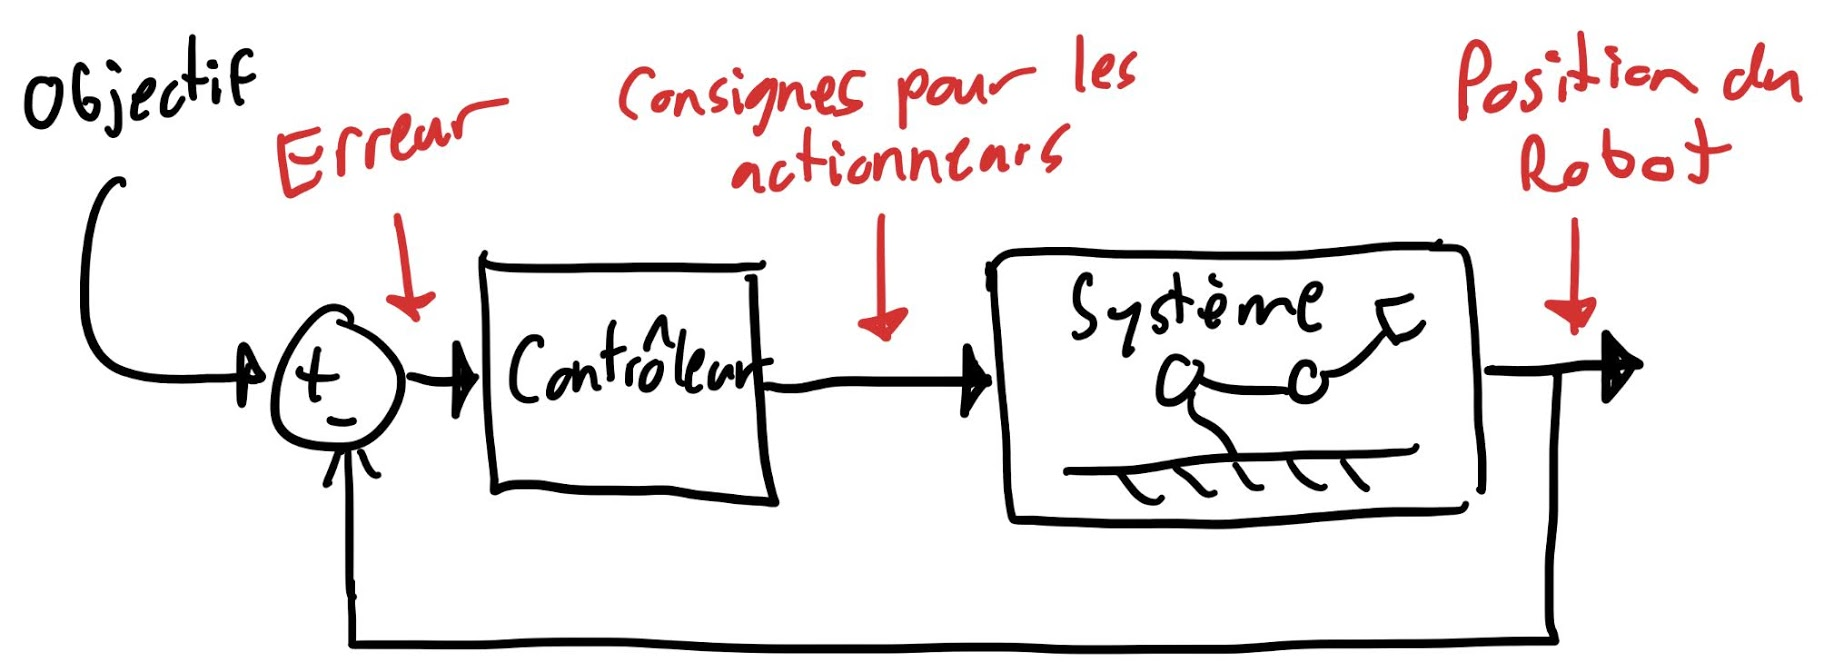
\includegraphics[width=0.7\textwidth]{fig/closedloop.jpg}
	\caption{Boucle fermée}
	\label{fig:closedloop}
\end{figure}
%%%%%%%%%%%%%%%%%%%%%%%%%%%%%%%%

Le principe de base d'une telle loi de commande peut se résumer à: si le système est trop à gauche pousse vers la droite et si le système est trop à droite pousse vers la gauche. Cette approche fonctionne bien pour des systèmes simples. Par exemple, pour contrôler la position d'un vérin électrique une loi de commande de type "pousse dans le sens inverse de l'erreur" est suffisante. Toutefois pour une voiture autonome, si la direction et la vitesse à prendre serait basée sur l'erreur totale, par exemple 150 km NW par rapport à la ville que l'on désire aller, la voiture tenterais de traverser des champs en ligne droite! Pour les systèmes plus compliqués, particulièrement avec des limites comme des obstacles, des saturations d'actionneurs, etc, le contrôleur n'est pas simplement une fonction de l'erreur.

Pour plusieurs systèmes robotiques, une loi de commande hybride est utilisée comme illustré à la Figure \ref{fig:trajectoryfollowingcontroller}. Un plan est déterminé comme avec l'approche en boucle ouverte, toutefois un contrôleur en boucle fermée qui agit sur l'erreur par rapport à la trajectoire cible est ensuite utilisé. La loi de commande dans ce cas, ne dépend pas seulement de la position actuel et de la position désirée, mais aussi du temps car elle compare la position actuelle à celle ou le robot doit théorique être rendu à ce moment. 
%%%%%%%%%%%%%%%%%%%%%%%%%%%%%%%%
\begin{figure}[htbp]
	\centering
		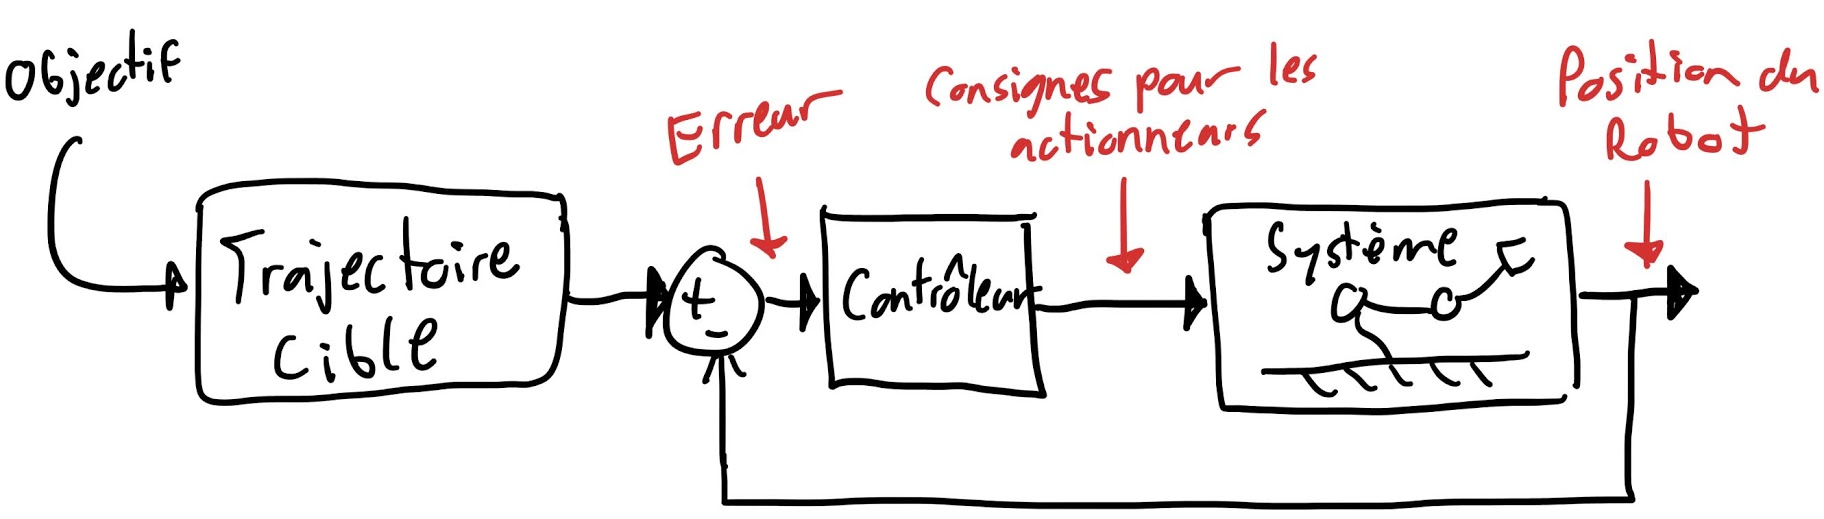
\includegraphics[width=0.8\textwidth]{fig/trajectoryfollowingcontroller.jpg}
	\caption{Contrôleur de suivi de trajectoire}
	\label{fig:trajectoryfollowingcontroller}
\end{figure}
%%%%%%%%%%%%%%%%%%%%%%%%%%%%%%%%



%%%%%%%%%%%%%%%%%%%%%%%%%%%%%%%%%%%%%%%%%%%%%%%%%%%%%%%%%%%%%%%%%%%%%%%%%%%%%%%%%%%%%%%%%%%%%%%%
\subsection{Boucles imbriquées}

La plupart des systèmes robotiques n'ont pas un seul gros contrôleur qui contrôle toutes les actions des actionneurs de façon centralisé, mais plutôt plusieurs sous-systèmes avec chacun des contrôleur locaux. Par exemple, lorsqu'un système robotisé utilise des servo-moteurs, l'électronique des moteurs inclus déjà un contrôleur qui effectue un asservissement en position ou en vitesse. 

Une architecture qui est souvent utilisée pour les robots manipulateur est illustrée à la Figure \ref{fig:innerloop}. Chaque joint du robot du robot a sont propre contrôleur en vitesse qui recoit une consigne d'un contrôleur central. Les contrôleurs locaux comparent la vitesse du joint désirée à une mesure de vitesse et détermine un couple moteur selon l'erreur en vitesse. Le contrôleur central lui compare la position cible à la position mesurée du robot et détermine le mouvement (consignes de vitesse) que les joints devraient faire pour corriger la position.
%%%%%%%%%%%%%%%%%%%%%%%%%%%%%%%%
\begin{figure}[htbp]
	\centering
		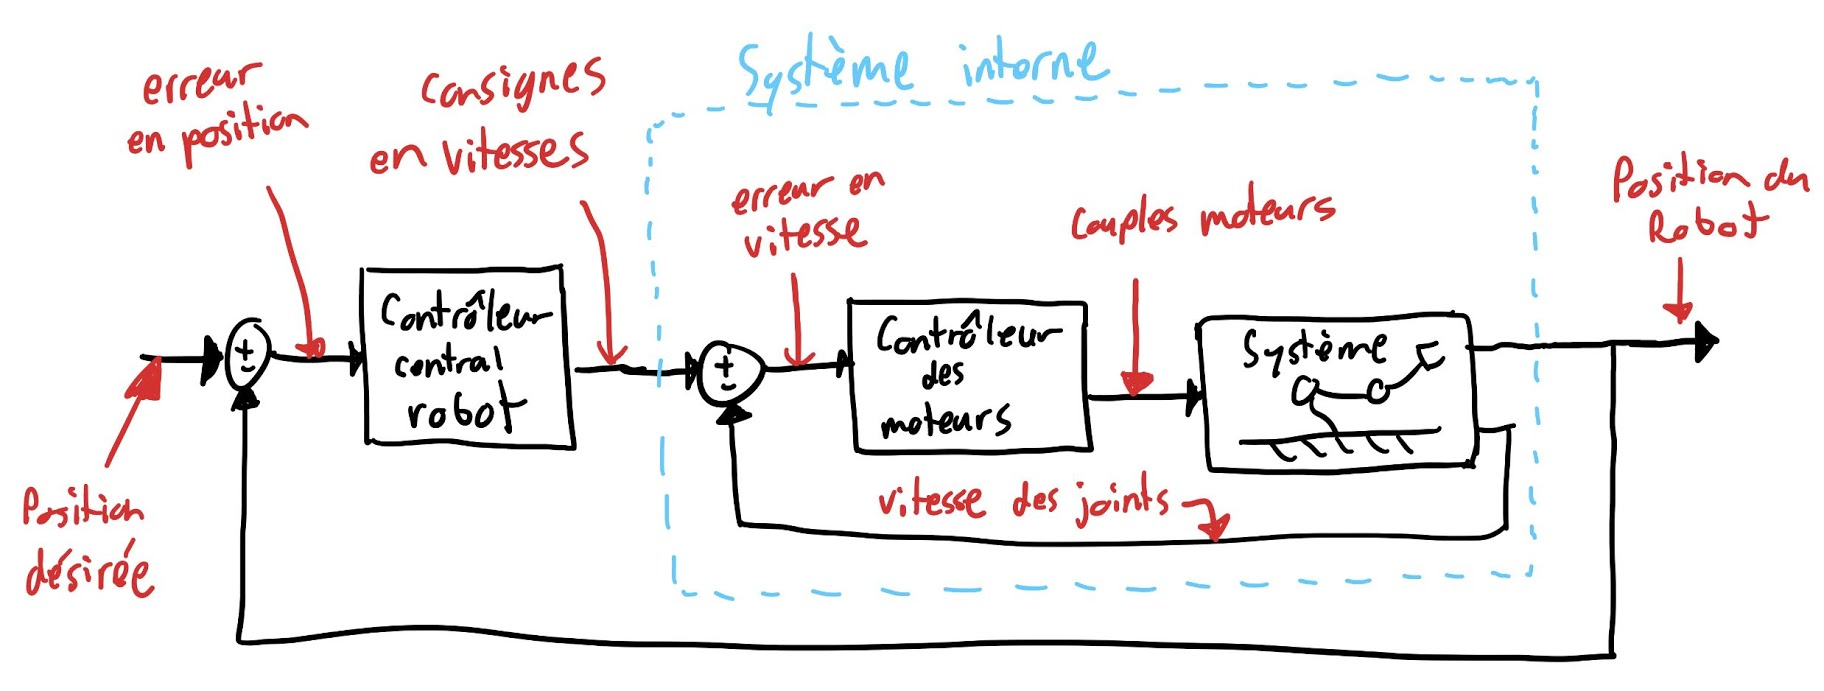
\includegraphics[width=0.9\textwidth]{fig/innerloop.jpg}
	\caption{Boucles imbriquées}
	\label{fig:innerloop}
\end{figure}
%%%%%%%%%%%%%%%%%%%%%%%%%%%%%%%%

Cette approche a comme avantage de découpler le problème en deux problèmes plus simples et rendre plus modulaires les loi de commande qui sont développée. Par exemple, le concepteur du contrôleur des moteurs pourrait effectuer sont travail sans ce soucier du modèle cinématique compliqué du bras manipulateur. Inversement, le concepteur du contrôleur central du robot pourrait travailler avec un modèle purement cinématique du robot (plutôt que les équations dynamiques qui relient les couples moteurs aux accélérations), en assumant que les boucles en vitesse des moteurs fonctionnent et sont rapide. Dans ces conditions, comme illustré à la Figure \ref{fig:innerloop2}, le concepteur du contrôleur central aurait un problème classique avec une seule boucle fermée, mais sont modèle du système considère les contrôleurs de moteurs. 

%%%%%%%%%%%%%%%%%%%%%%%%%%%%%%%%
\begin{figure}[htbp]
	\centering
		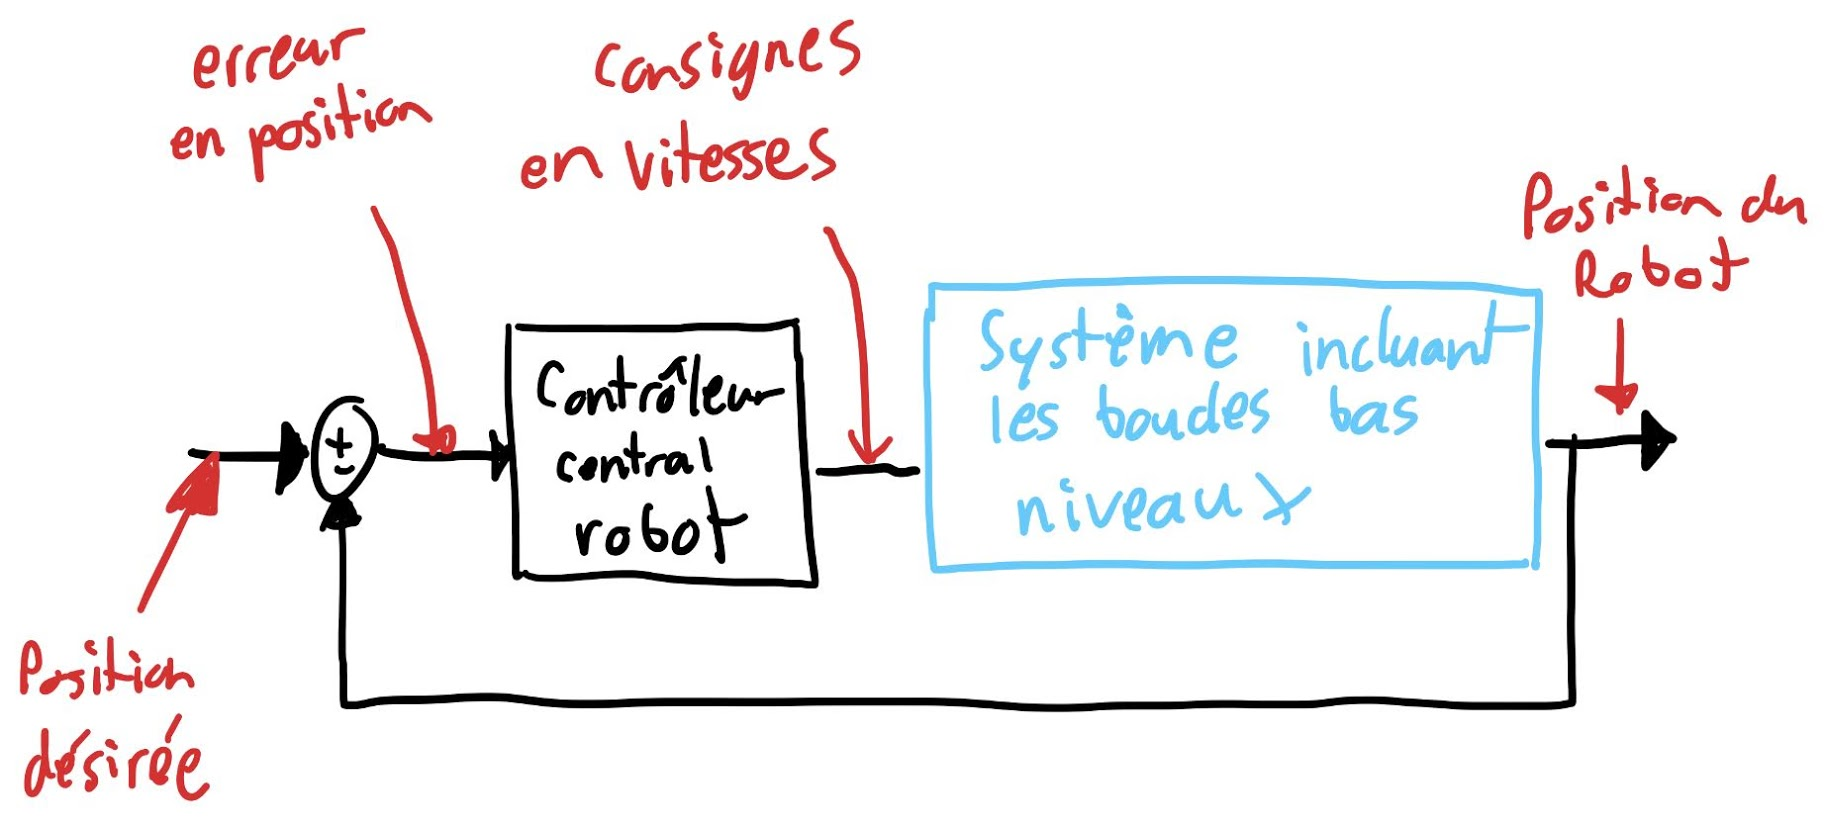
\includegraphics[width=0.7\textwidth]{fig/innerloop2.jpg}
	\caption{Boucle fermée du contrôleur central}
	\label{fig:innerloop2}
\end{figure}
%%%%%%%%%%%%%%%%%%%%%%%%%%%%%%%%

Il est donc important de noté que le modèle utilisé pour la conception du ou des contrôleurs d'un système robotisé doit être adapté au contexte et à l'architecture utilisée. 


%%%%%%%%%%%%%%%%%%%%%%%%%%%%%%%%%%%%%%%%%%%%%%%%%%%%%%%%%%%%%%%%%%%%%%%%%%%%%%%%%%%%%%%%%%%%%%%%
\subsection{Synthétisation d'un plan hors-ligne ou en-ligne}

Un autre aspect pour les méthodes de commandes avancées qui utilise beaucoup de calculs numériques, est qu'est-ce qui est calculé d'avance vs. en temps réel durant l'exécution du contrôleur. 

Une architecture souvent utilisée avec les algorithmes de planification/optimisation de trajectoire (ex. RRT) est illustrée à la Figure \ref{fig:offlinetrajectorygeneration}. Les calculs lourds de rechercher et/ou optimisation sont effectués d'avance, et lors de l'exécution la loi de commande utilise seulement la trajectoire cible qui a été synthétisée hors-ligne.
%%%%%%%%%%%%%%%%%%%%%%%%%%%%%%%%
\begin{figure}[htbp]
	\centering
		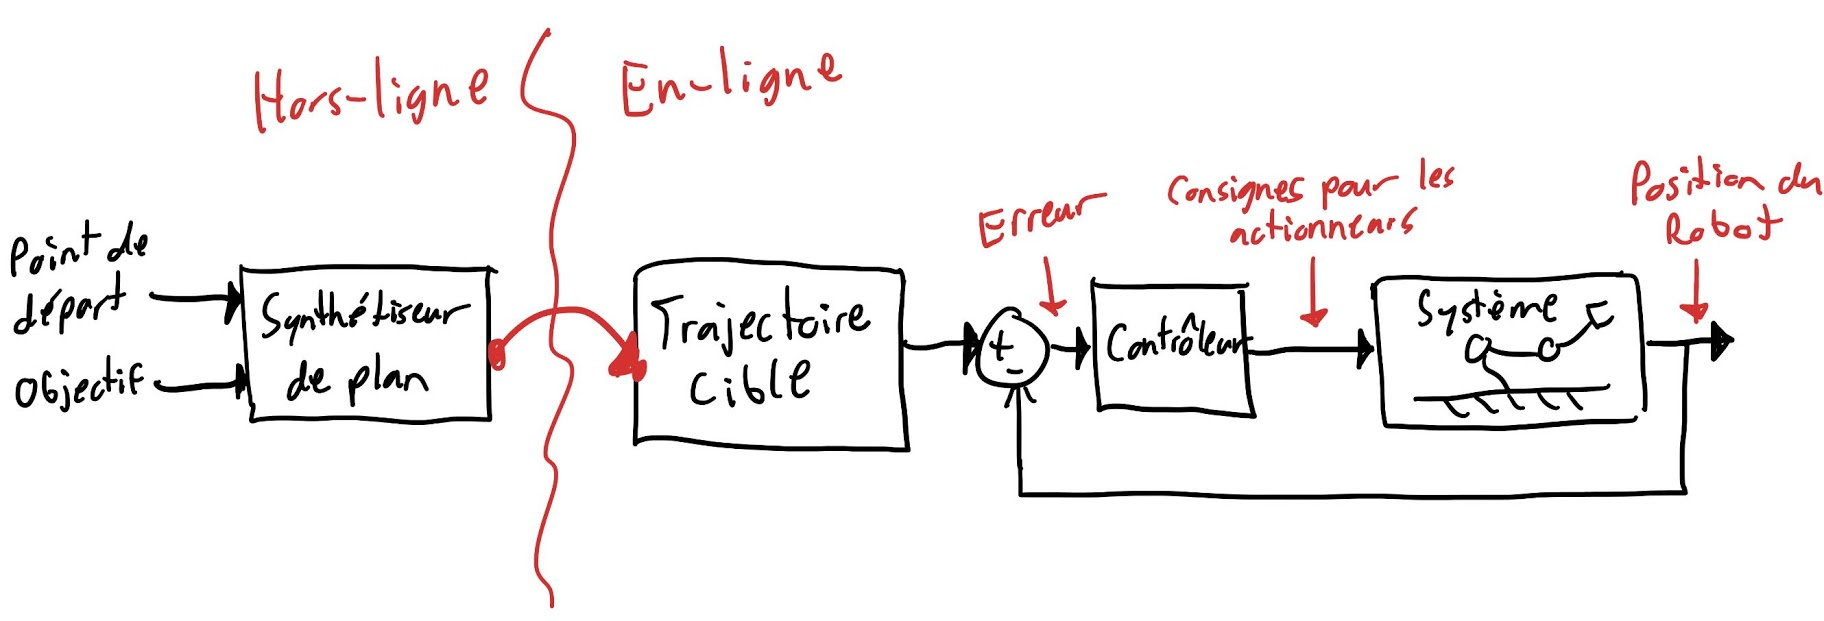
\includegraphics[width=0.9\textwidth]{fig/offlinetrajectorygeneration.jpg}
	\caption{Générateur de trajectoire hors-ligne}
	\label{fig:offlinetrajectorygeneration}
\end{figure}
%%%%%%%%%%%%%%%%%%%%%%%%%%%%%%%%

De façon similaire, les méthodes comme \textit{LQR} ou bien \textit{value-iteration} effectue des calculs généralement hors-ligne pour synthétisé une loi de commande sous forme de carte $\col{u} = c(\col{x})$ de quelles actions $\col{u}$ prendre en fonction des états mesurés $\col{x}$ du robot. C'est donc ici une fonction qui est synthétisée hors-ligne et utilisée en-ligne, voir Figure \ref{fig:offlinecontrollergeneration}. La fonction synthétisée peut-être analytique, par exemple pour la méthode \textit{LQR} avec un format $\col{u} = K \col{x}$, ou bien numérique, comme par exemple pour un contrôleur synthétisé avec la méthode \textit{value-iteration}. 
%%%%%%%%%%%%%%%%%%%%%%%%%%%%%%%%
\begin{figure}[htbp]
	\centering
		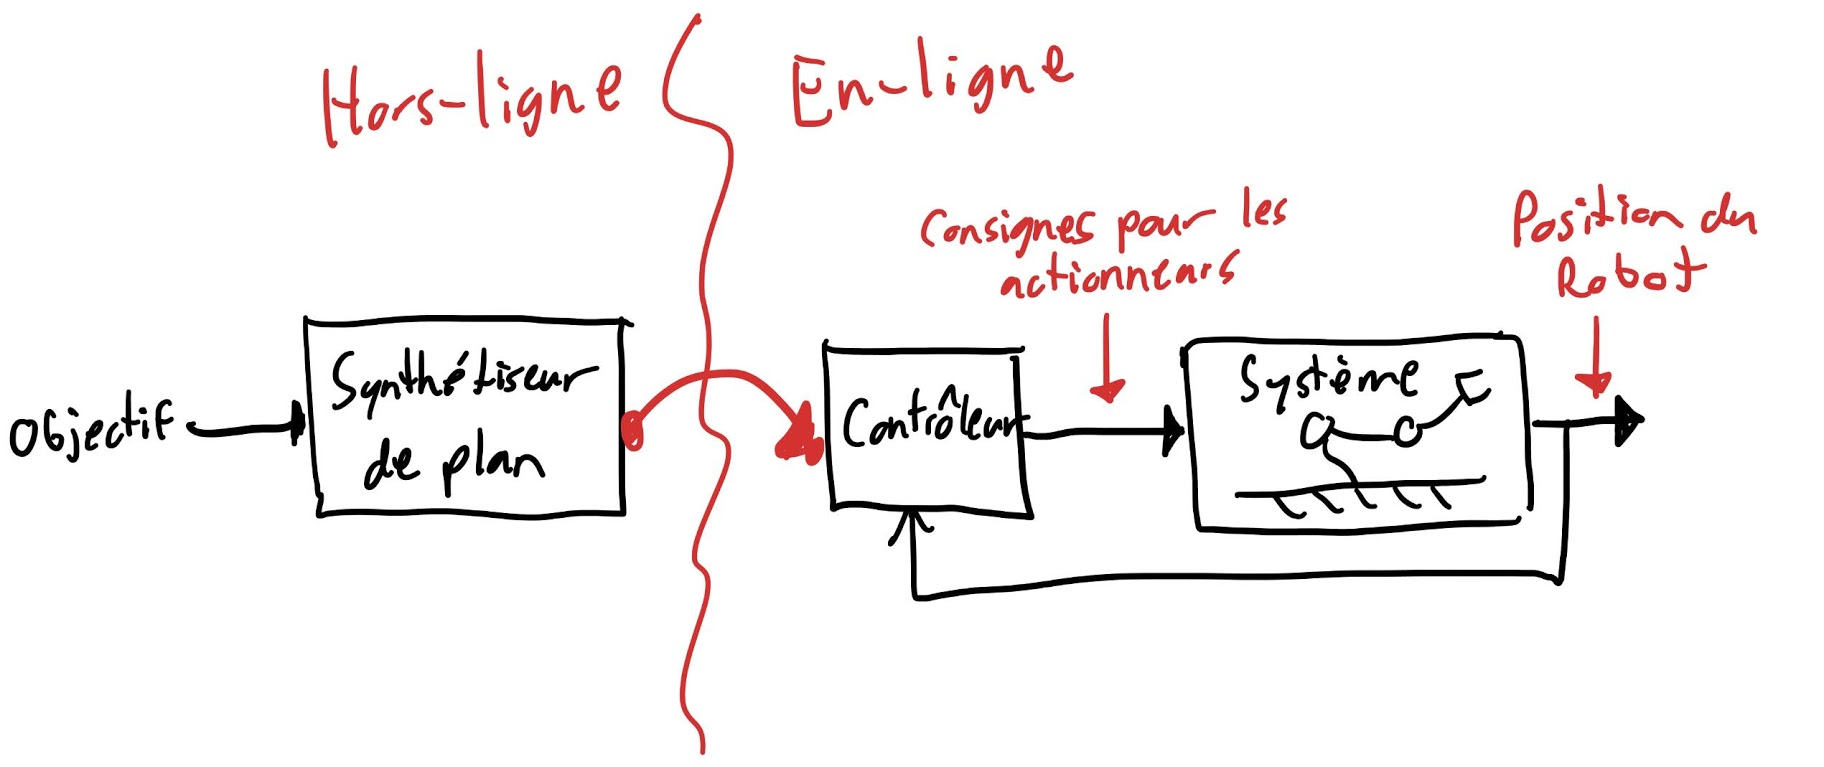
\includegraphics[width=0.9\textwidth]{fig/offlinecontrollergeneration.jpg}
	\caption{Génération de contrôleur hors-ligne}
	\label{fig:offlinecontrollergeneration}
\end{figure}
%%%%%%%%%%%%%%%%%%%%%%%%%%%%%%%%

Ensuite, certain type de contrôleurs de systèmes robotiques vont avoir une certaine forme de synthétisation de trajectoire ou de contrôleur mais en ligne, voir un exemple à la Figure \ref{fig:onlinetrajectorygeneration}. Typiquement, du au lourd calcul numérique qui doivent être fait en ligne, les architectures vont aussi utilisée des boucles imbriquée avec une boucle interne plus rapide et une boucle externe plus lente qui met à jour la trajectoire cible. L'approche de commande prédictive (MPC Model Predictive Control), est un exemple ou on optimise des trajectoire cible constament en ligne dans la boucle. 
%%%%%%%%%%%%%%%%%%%%%%%%%%%%%%%%
\begin{figure}[htbp]
	\centering
		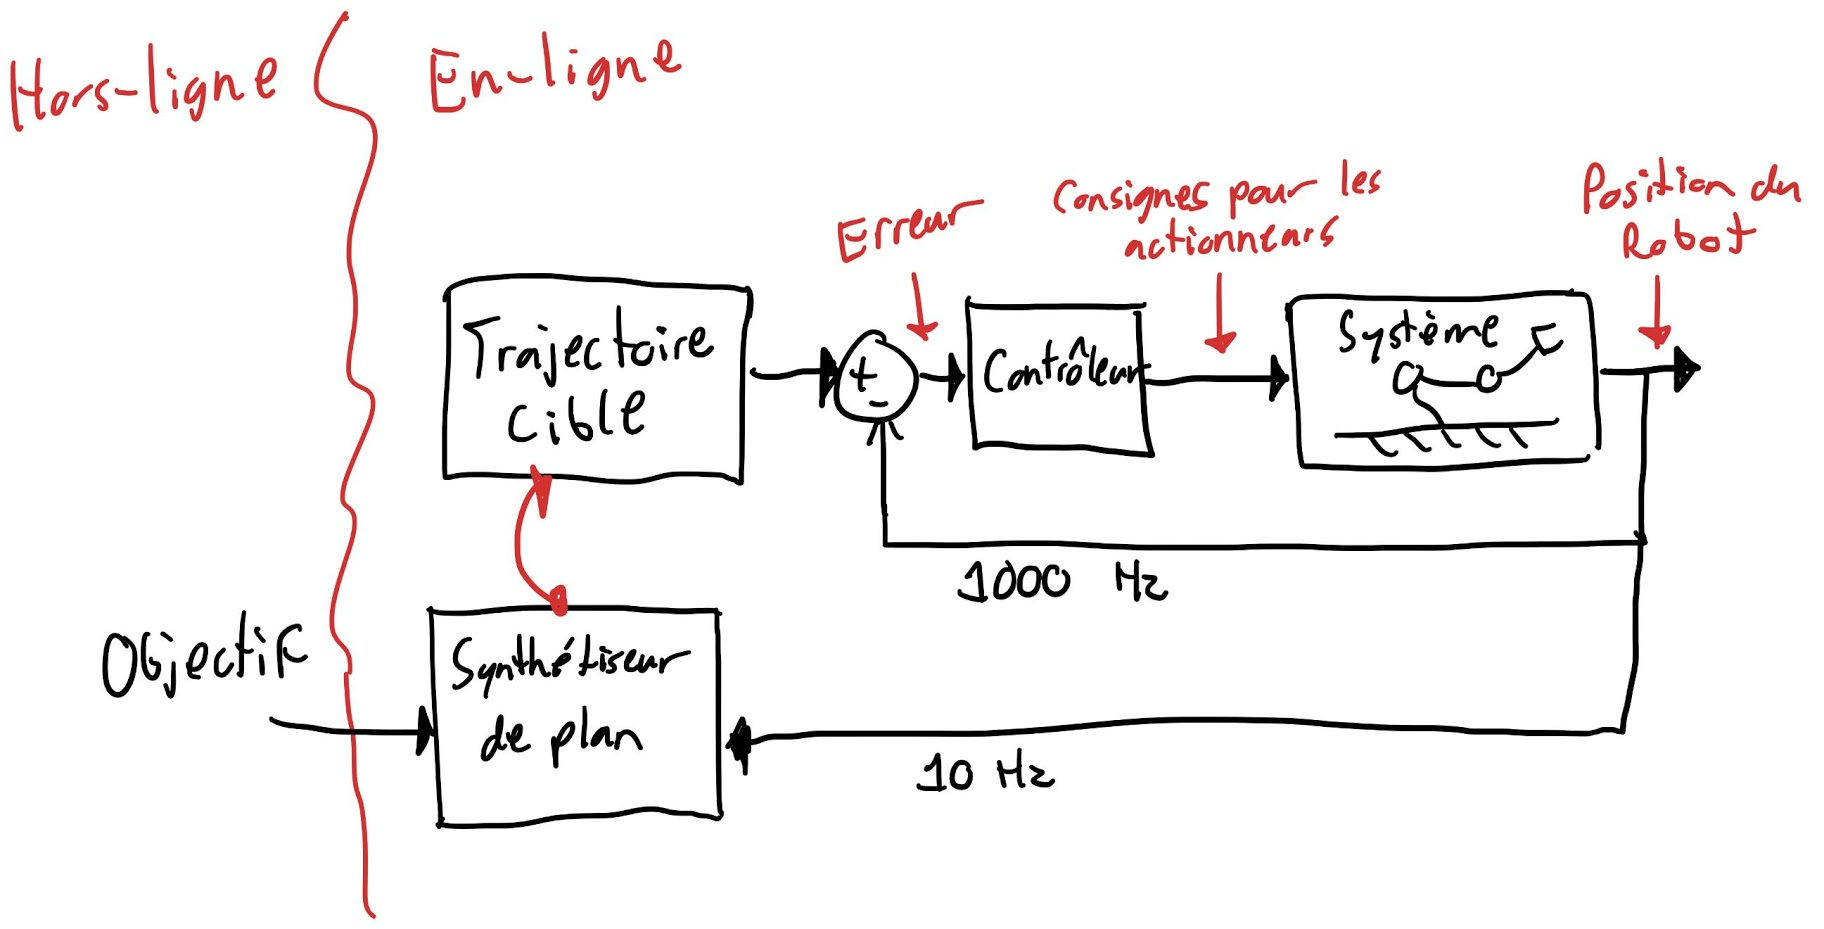
\includegraphics[width=0.9\textwidth]{fig/onlinetrajectorygeneration.jpg}
	\caption{Génération de trajectoire en ligne}
	\label{fig:onlinetrajectorygeneration}
\end{figure}
%%%%%%%%%%%%%%%%%%%%%%%%%%%%%%%%




%\section{Boucle ouverte vs. boucle fermée}
%\label{sec:BoucleOuverteVsBoucleFermée}


% \begin{figure}[htbp]
% 	\centering
% 		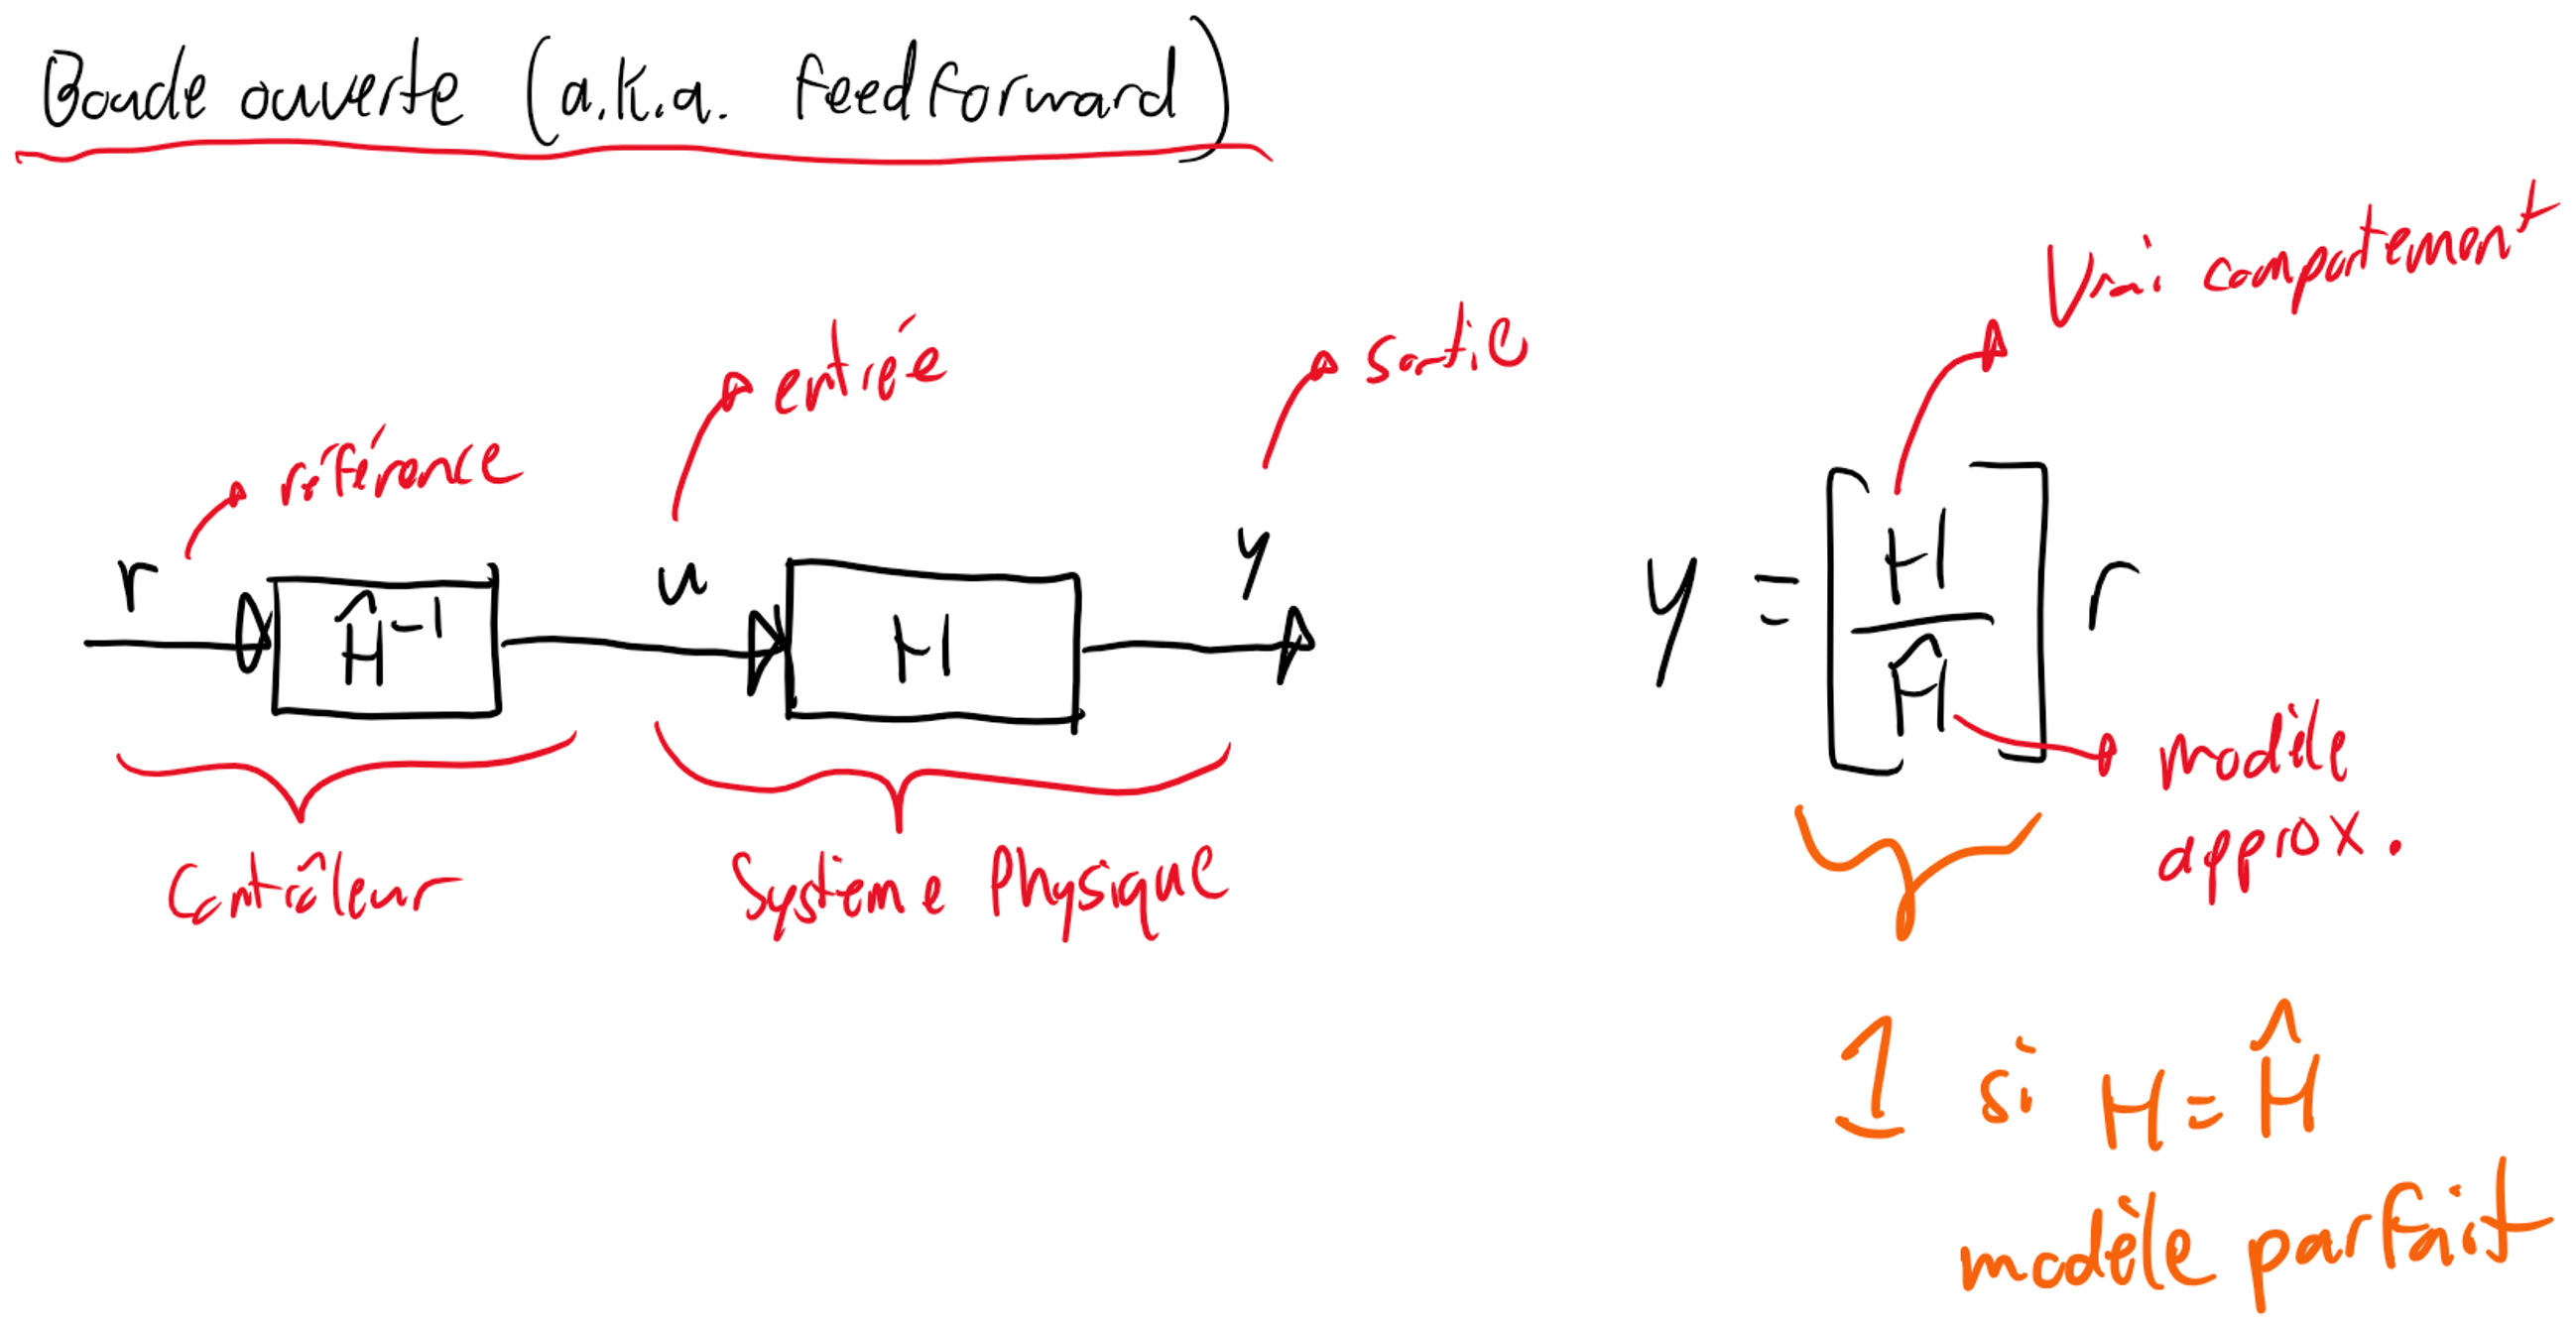
\includegraphics[width=1.00\textwidth]{boucleouverte.png}
% 	\caption{Boucle ouverte}
% 	\label{fig:boucleouverte}
% \end{figure}
